\section{Part-based R-CNNs}
\label{sec:recursive-part-dets}

While~\cite{rcnn} demonstrated the effectiveness of the R-CNN method on a generic object detection task (PASCAL VOC), it did not explore the application of this method to simultaneous localization and fine-grained recognition.
%Fine-grained recognition demands more than a coarse shape estimate of an object category due to the high semantic similarity of object categories, such as different species of birds.
Because our work operates in this regime, we extend R-CNN to detect objects and localize their parts under a geometric prior.
With hypotheses for the locations of individual semantic parts of the object of interest (e.g., the location of the head for an animal class), it becomes reasonable to model subtle appearance differences which tend to appear in locations that are roughly fixed with respect to these parts.

In the R-CNN method, for a particular object category, a candidate detection $x$ with CNN feature descriptor $\phi(x)$ is assigned a score of $w_0^{\intercal} \phi(x)$, where $w_0$ is the learned vector of SVM weights for the object category.
In our method, we assume a strongly supervised setting (e.g., \cite{Hossein_ECCV12}) in which at training time we have ground truth bounding box annotations not only for full objects, but for a fixed set of semantic parts $\{p_1, p_2, ..., p_n\}$ as well.

Given these part annotations, at training time all objects and each of their parts are initially treated as independent object categories: we train a one-versus-all linear SVM on feature descriptors extracted over region proposals, where regions with $\ge 0.7$ overlap with a ground truth object or part bounding box are labeled as positives for that object or part, and regions with $\le 0.3$ overlap with any ground truth region are labeled as negatives.
Hence for a single object category we learn whole-object (``root'') SVM weights $w_0$ and part SVM weights $\{w_1, w_2, ..., w_n\}$ for parts $\{p_1, p_2, ..., p_n\}$ respectively.
At test time, for each region proposal window we compute scores from all root and part SVMs.
Of course, these scores do not incorporate any knowledge of how objects and their parts are constrained geometrically; for example, without any additional constraints the \textit{bird head} detector may fire outside of a region where the \textit{bird} detector fires.
% for any response from a \textit{bird} detector, we should see a corresponding high score for a smaller window somewhere inside of the region from the \textit{bird head} detector.
Hence our final joint object and part hypotheses are computed using the geometric scoring function detailed in the following section, which enforces the intuitively desirable property that pose predictions are consistent with the statistics of poses observed at training time.

\subsection{Geometric constraints}
Let $X =\{x_0, x_1, \ldots, x_n\}$ denote the locations (bounding boxes) of object $p_0$ and $n$ parts $\{p_i\}_{i=1}^n$, which are annotated in the training data, but unknown at test time. Our goal is to infer both the object location and part locations in a previously unseen test image. Given the R-CNN  weights $\{w_0, w_1, \ldots, w_n\}$ for object and parts, we will have the corresponding detectors $\{d_0, d_1, \ldots, d_n\}$ where each detector score is $d_i(x) = \sigma(w_i^{\intercal} \phi(x))$, where $\sigma(\cdot)$ is the sigmoid function and $\phi(x)$ is the CNN feature descriptor extracted at location $x$.
We infer the joint configuration of the object and parts by solving the following optimization problem:
\begin{equation}
X^* = \arg \max_{X}
\Delta(X)
\prod_{i=0}^n d_i(x_i)
\end{equation}
where $\Delta(X)$ defines a scoring function over the joint configuration of the object and root bounding box.
% , and $\alpha$ is a hyperparameter controlling the weight of this scoring function versus the detector scores.
We consider and report quantitative results on several configuration scoring functions $\Delta$, detailed in the following paragraphs.

% where $c_x(y)$ is true if and only if region $y$ falls inside region $x$.
% In our experiments, we relax these constraints slightly by allowing part boxes with edges outside of the whole object window by a maximum of 10 pixels.
% However, as the individual part detectors are less than perfect, the window with highest individual part detector scores are not always correct, especially when there are occlusions.
% We therefore consider the following two scoring functions to enforce constraints over the layout of the parts relative to the object location to filter out incorrect detections.

\paragraph{Box constraints.}
One intuitive idea to localize both the object and parts is to consider each possible object window and all the windows inside the object and pick the windows with the highest part scores.
In this case, we define the scoring function
\begin{equation}
\Delta_{\mathrm{box}}(X) = \prod_{i=1}^n c_{x_0}(x_i)
\end{equation}
where
\begin{equation}
c_x(y) =
\left\{
\begin{array}{ll}
1 & \text{if region } y \text{ falls outside region } x \text{ by at most } \epsilon \text{ pixels }\\
0 & \text{otherwise}
\end{array}
\right.
\end{equation}
In our experiments, we let $\epsilon = 10$.
%\todo{``falls outside region...'' is too imprecise. Shouldn't $\epsilon$ be a scale-free quantity?}

\paragraph{Geometric constraints.}
Because the individual part detectors are less than perfect, the window with highest individual part detector scores is not always correct, especially when there are occlusions.
We therefore consider several scoring functions to enforce constraints over the layout of the parts relative to the object location to filter out incorrect detections.
We define
\begin{equation}
\Delta_{\mathrm{geometric}}(X) = \Delta_{\mathrm{box}}(X) \left( \prod_{i=1}^n \delta_i(x_i) \right)^{\alpha}
\end{equation}
where
% $\Theta = \{\theta_k\}$ is the set of exemplars and
$\delta_i$ is a scoring function for the position of the part $p_i$ given the training data. %given the exemplars $\Theta$.\todo{Exemplars not previously defined...seems out of place.}
Following previous work on part localization from, e.g.~\cite{belkrieg,dpm,pictorial},
we experiment with three definitions of $\delta$:
\begin{itemize}
%\item
%$\delta_i^{G}(x_i)$ fits a simple Gaussian model to the training data for the placement $x_i$ of part $p_i$ relative to the whole object placement $x_0$. \ning{Maybe we should remove this since we don't include $\delta^{G}$ in the experiment section.}
%\vspace{0.3cm}

\item
$\delta_i^{MG}(x_i)$ fits a mixture of Gaussians model with $N_g$ components to the training data for part $p_i$.  In our experiments, we set $N_g = 4$.
%\vspace{0.3cm}

\item
$\delta_i^{NP}(x_i)$ finds the $K$ nearest neighbors in appearance space to
$\tilde{x}_0$, where $\tilde{x}_0 = \arg \max d_0(x_0)$ is the top-scoring window from the root detector.
We then fit a Gaussian model to these $K$ neighbors.
In our experiments, we set $K = 20$. Figure \ref{fig:np} illustrates some examples of nearest neighbors. 
\end{itemize}

The DPM~\cite{dpm} models deformation costs with a per-component Gaussian prior. R-CNN~\cite{rcnn} is a single-component model, motivating the $\delta^{MG}$ or $\delta^{NP}$ definitions.
Our $\delta^{NP}$ definition is inspired by Belhumeur et al.~\cite{belkrieg}, but differs in that we index nearest neighbors on appearance rather than geometry.


\begin{figure*}
\begin{center}
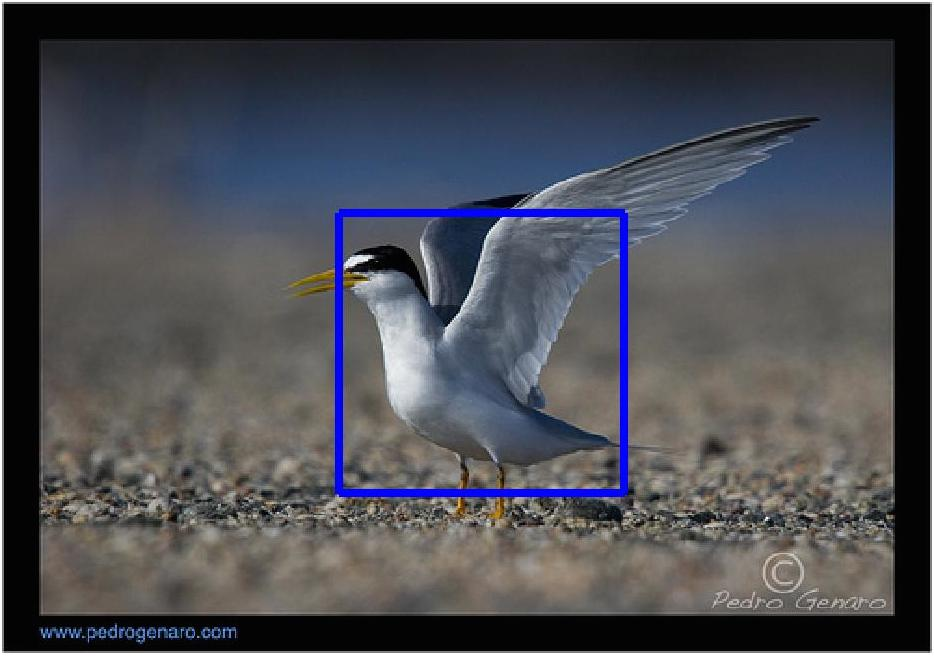
\includegraphics[width=0.15\linewidth, height = 0.1\linewidth]{1_orginal.jpg} 
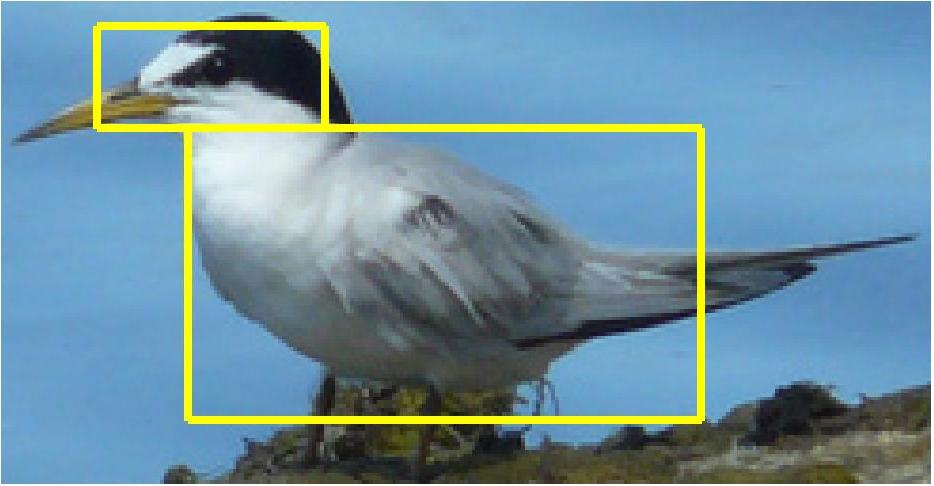
\includegraphics[width=0.15\linewidth, height = 0.1\linewidth]{1_1.jpg} 
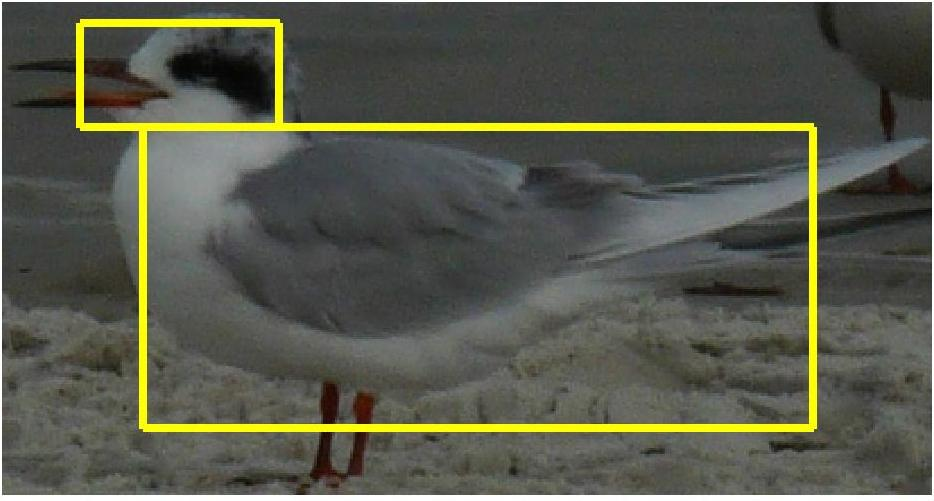
\includegraphics[width=0.15\linewidth, height = 0.1\linewidth]{1_2.jpg} 
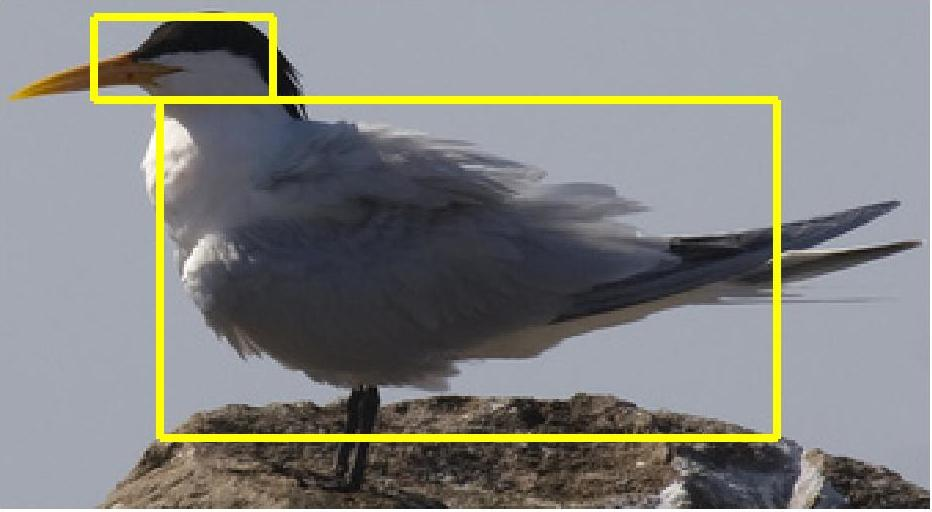
\includegraphics[width=0.15\linewidth, height = 0.1\linewidth]{1_3.jpg} 
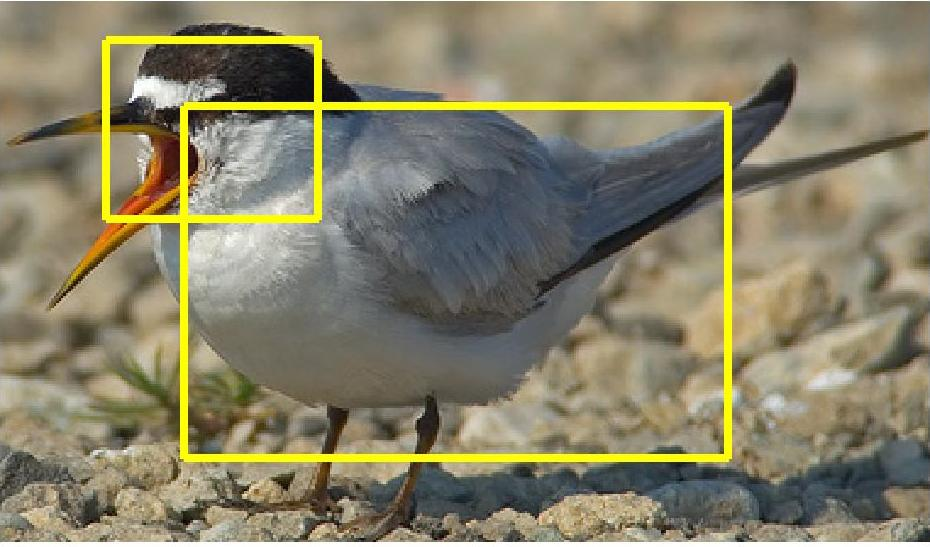
\includegraphics[width=0.15\linewidth, height = 0.1\linewidth]{1_4.jpg} 
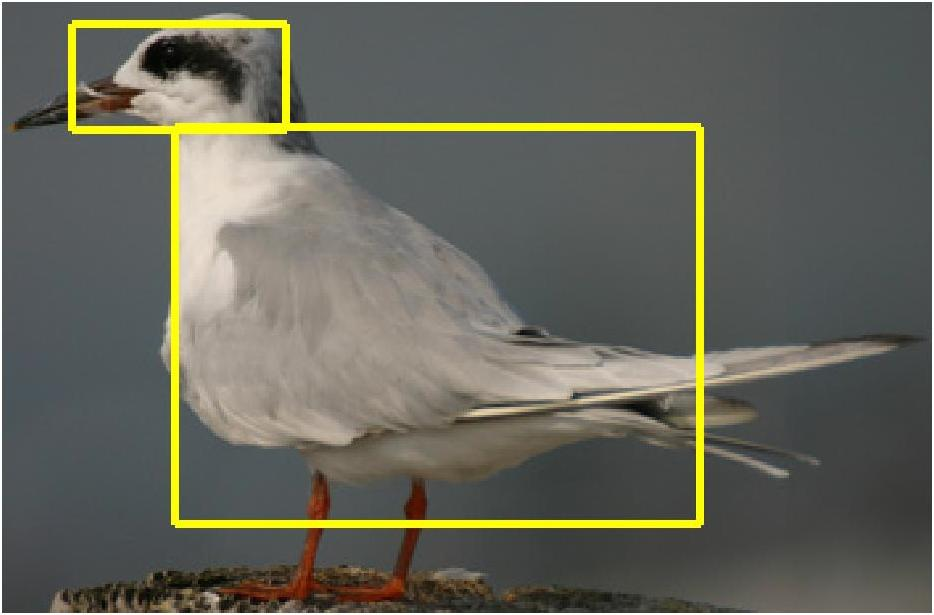
\includegraphics[width=0.15\linewidth, height = 0.1\linewidth]{1_5.jpg} 
\\
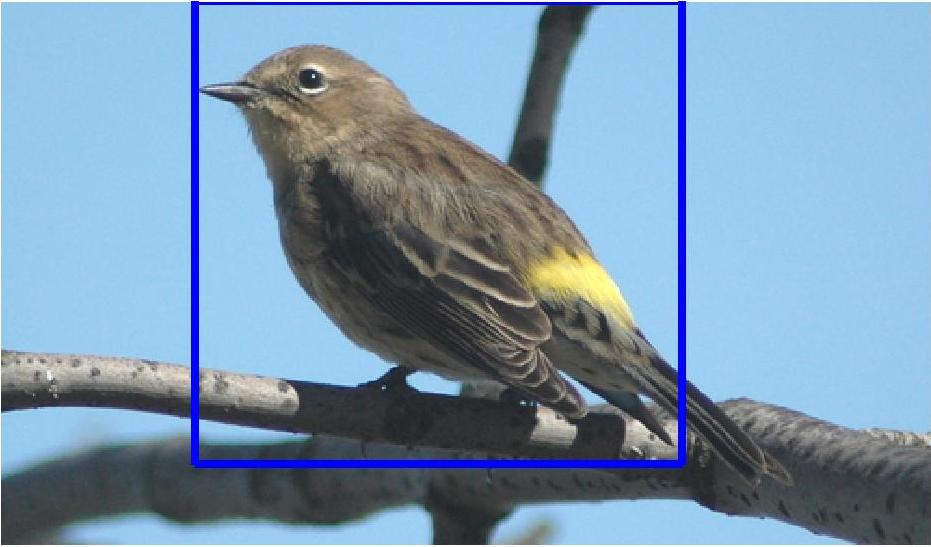
\includegraphics[width=0.15\linewidth, height = 0.1\linewidth]{2_orginal.jpg} 
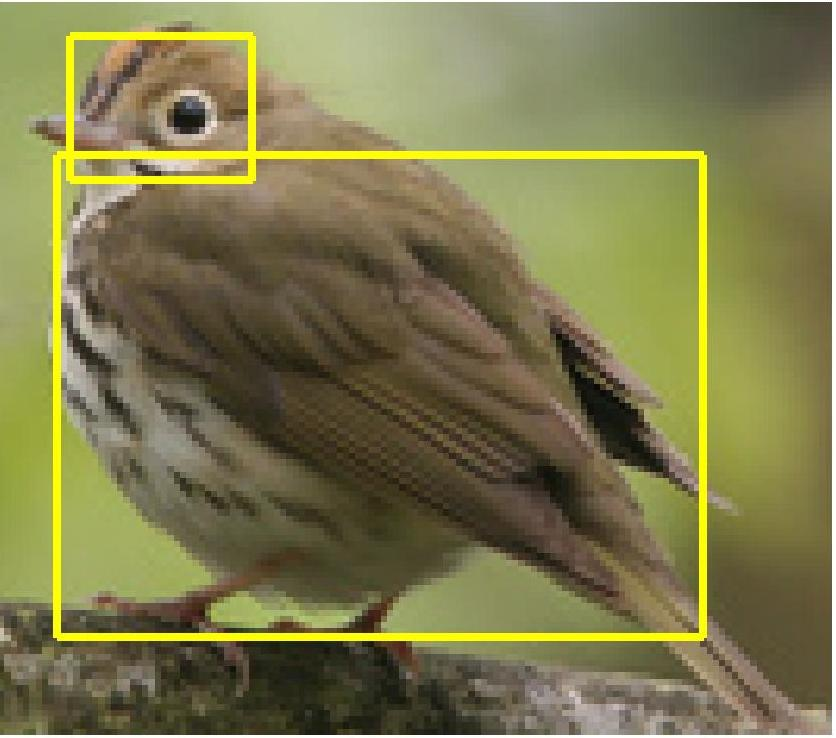
\includegraphics[width=0.15\linewidth, height = 0.1\linewidth]{2_1.jpg} 
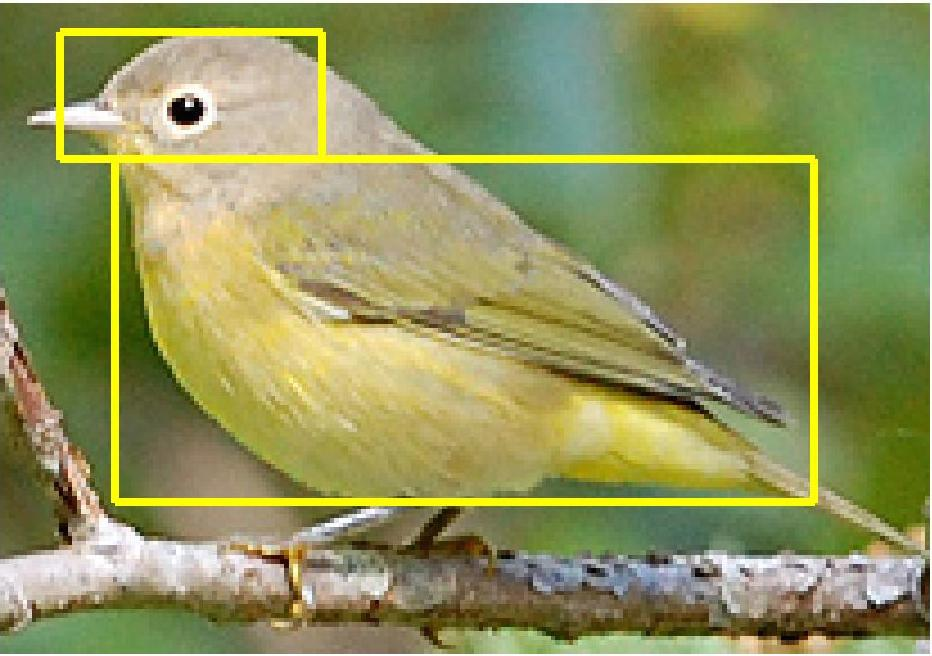
\includegraphics[width=0.15\linewidth, height = 0.1\linewidth]{2_2.jpg} 
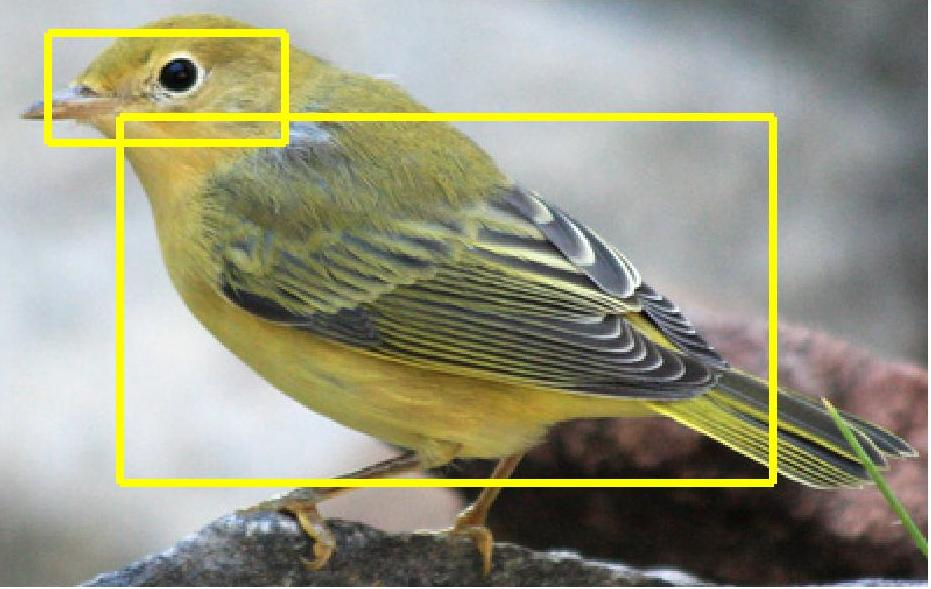
\includegraphics[width=0.15\linewidth, height = 0.1\linewidth]{2_3.jpg} 
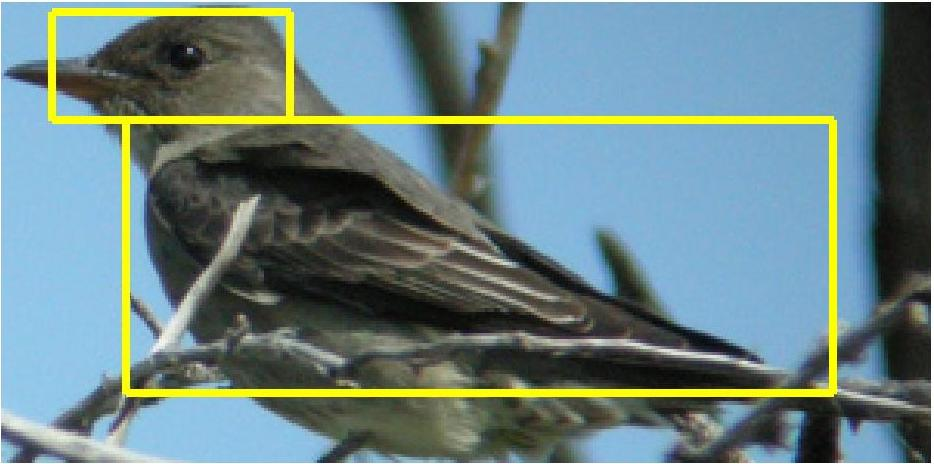
\includegraphics[width=0.15\linewidth, height = 0.1\linewidth]{2_4.jpg} 
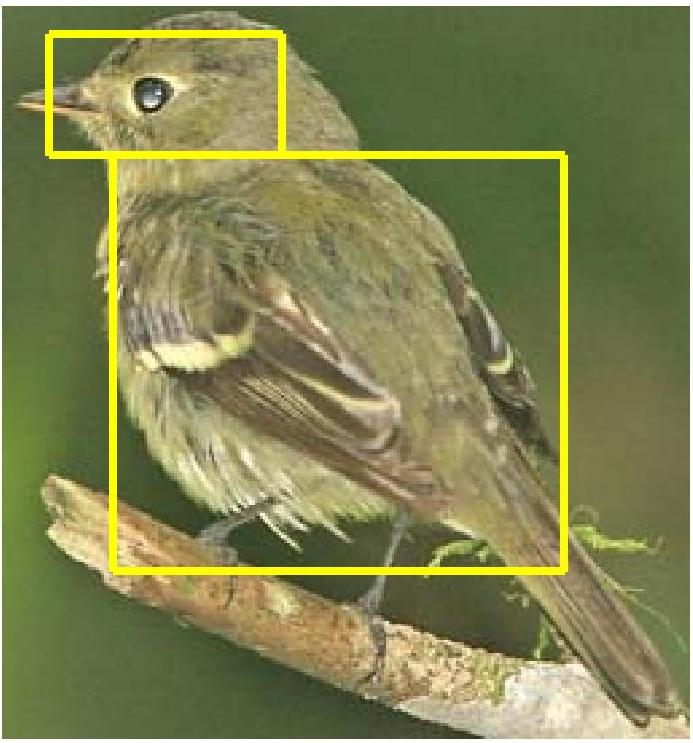
\includegraphics[width=0.15\linewidth, height = 0.1\linewidth]{2_5.jpg} 
\\
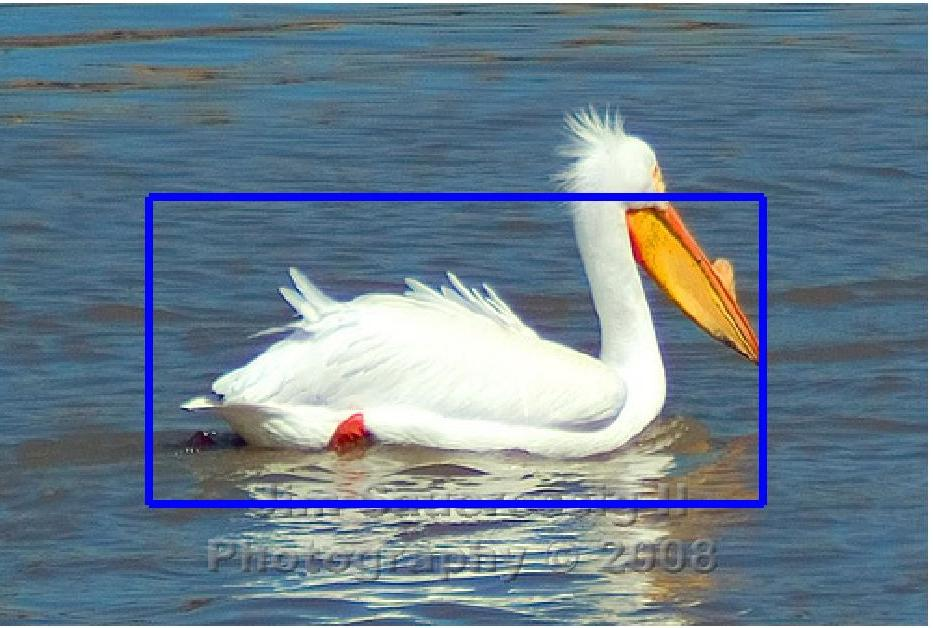
\includegraphics[width=0.15\linewidth, height = 0.1\linewidth]{6_orginal.jpg} 
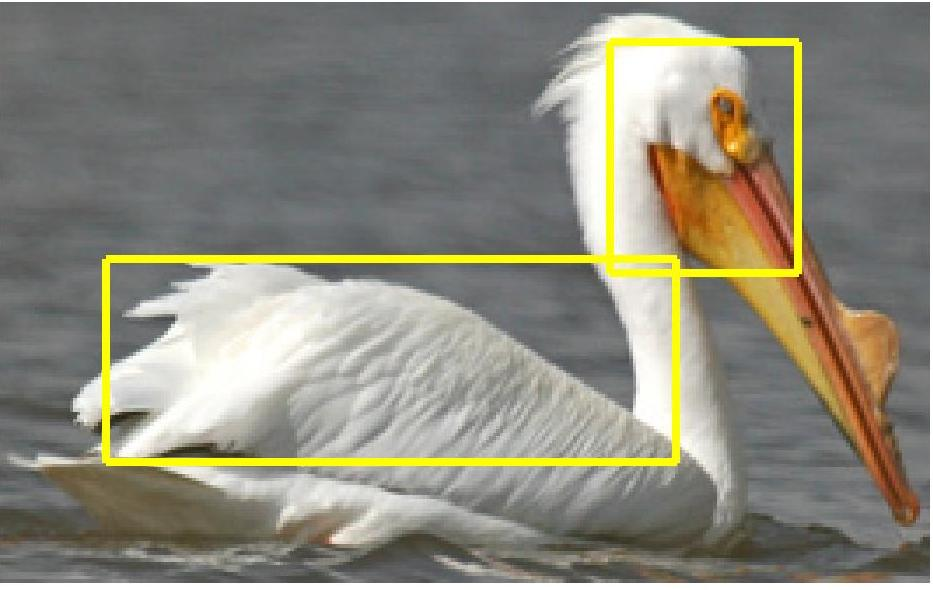
\includegraphics[width=0.15\linewidth, height = 0.1\linewidth]{6_1.jpg} 
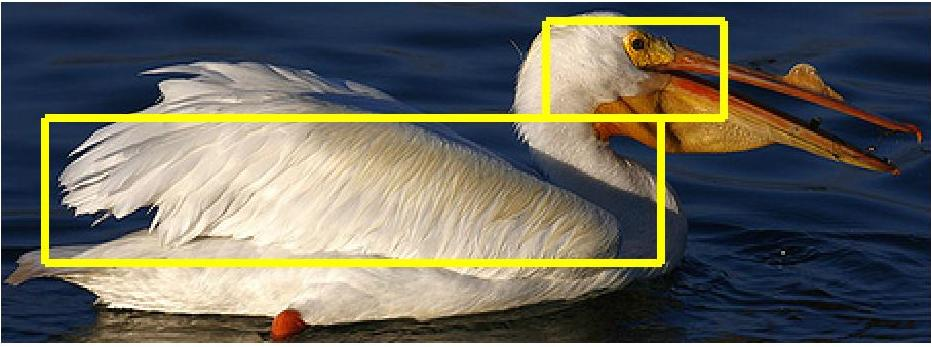
\includegraphics[width=0.15\linewidth, height = 0.1\linewidth]{6_2.jpg} 
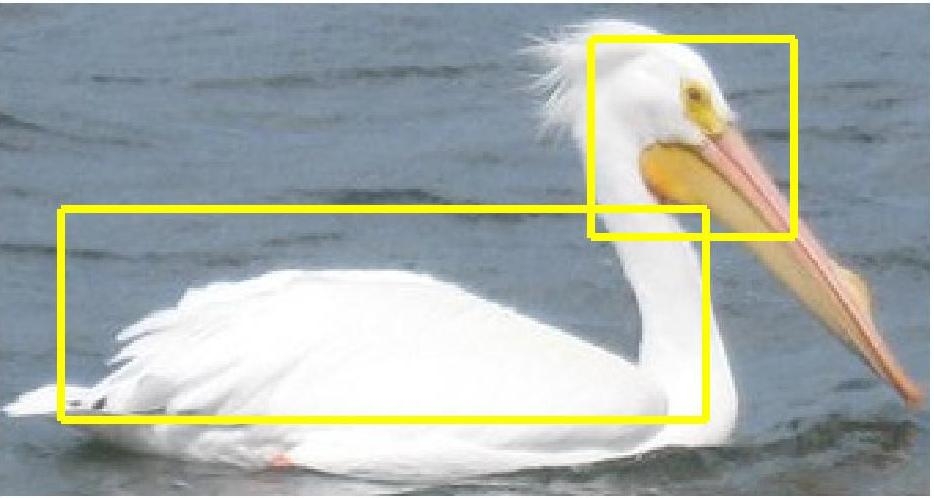
\includegraphics[width=0.15\linewidth, height = 0.1\linewidth]{6_3.jpg} 
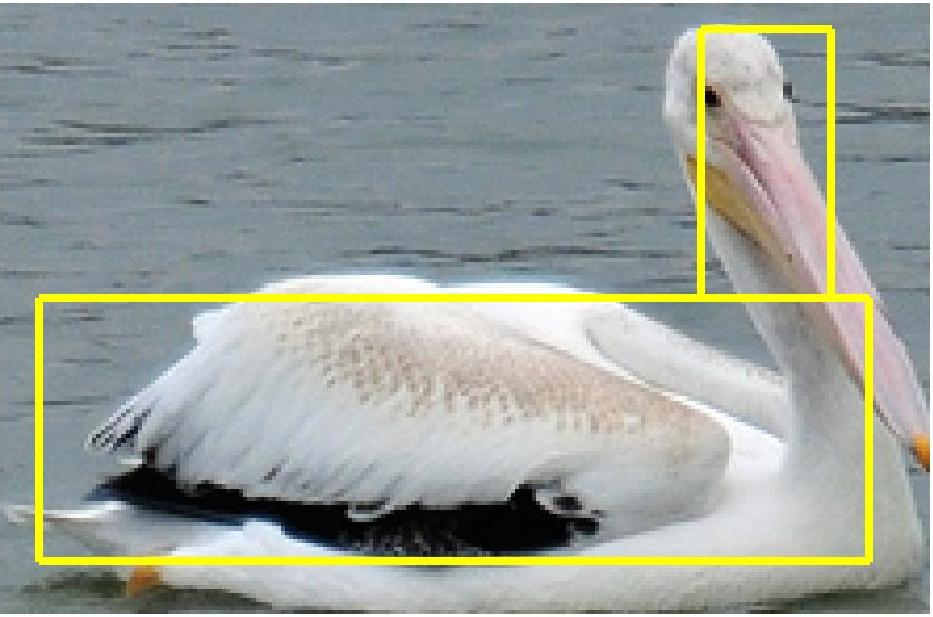
\includegraphics[width=0.15\linewidth, height = 0.1\linewidth]{6_4.jpg} 
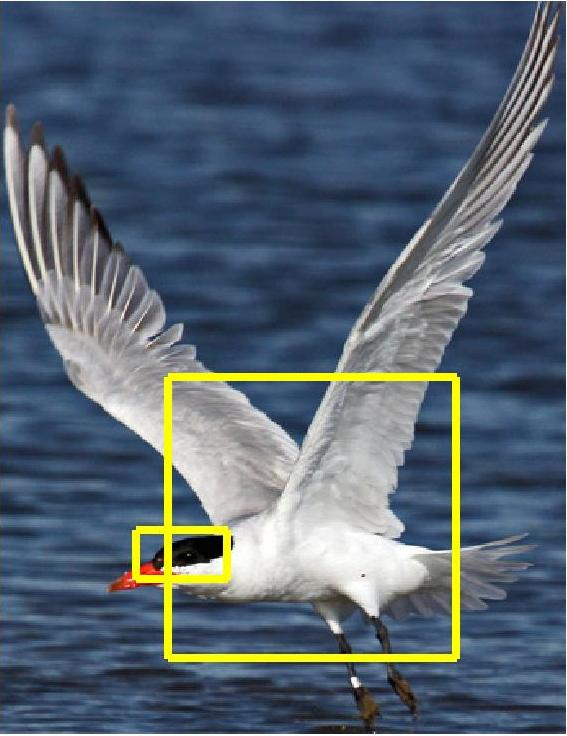
\includegraphics[width=0.15\linewidth, height = 0.1\linewidth]{6_5.jpg} 
\\
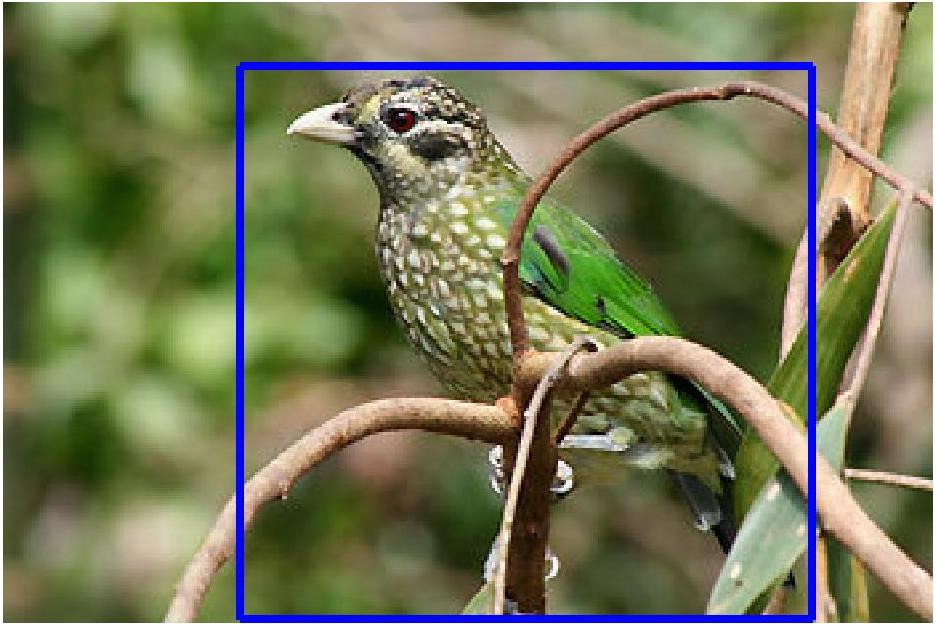
\includegraphics[width=0.15\linewidth, height = 0.1\linewidth]{8_orginal.jpg} 
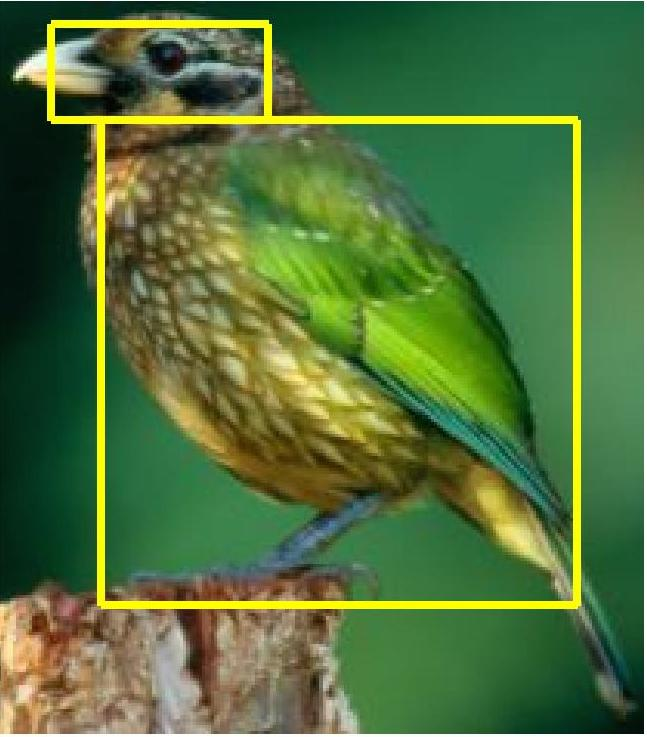
\includegraphics[width=0.15\linewidth, height = 0.1\linewidth]{8_1.jpg} 
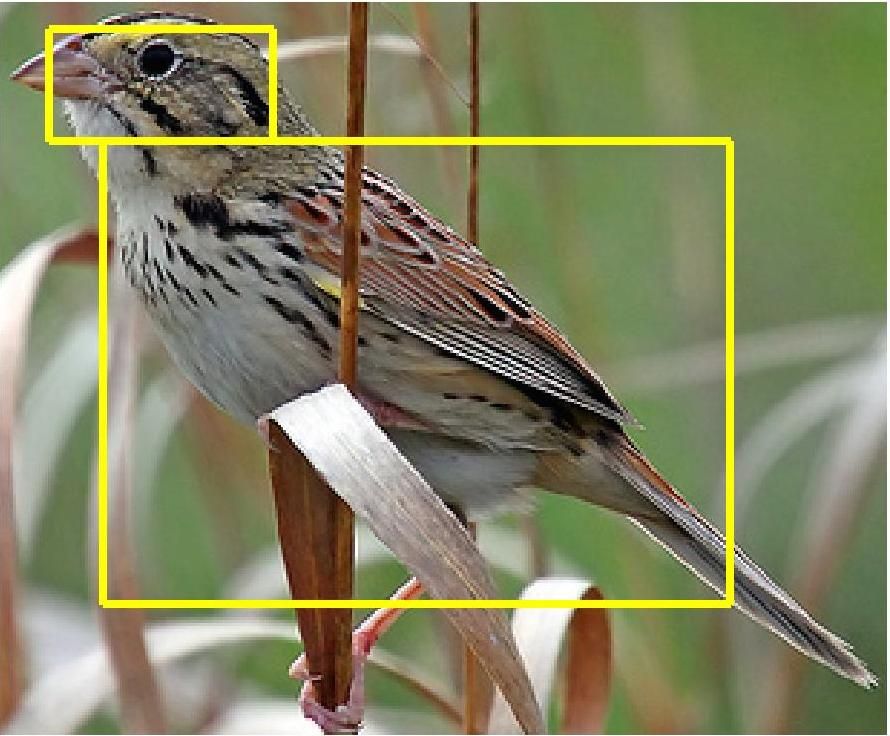
\includegraphics[width=0.15\linewidth, height = 0.1\linewidth]{8_2.jpg} 
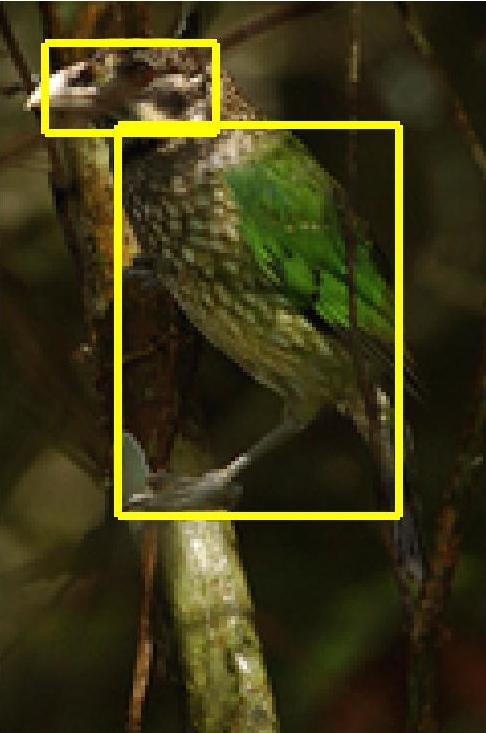
\includegraphics[width=0.15\linewidth, height = 0.1\linewidth]{8_3.jpg} 
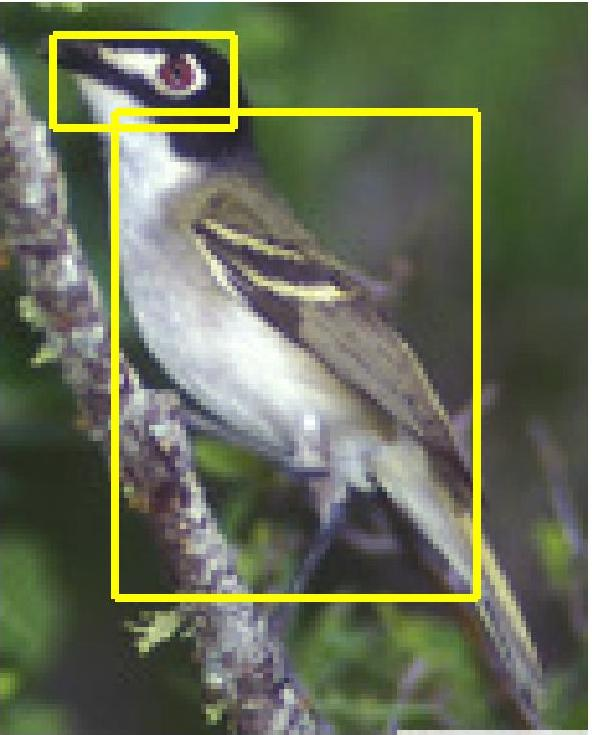
\includegraphics[width=0.15\linewidth, height = 0.1\linewidth]{8_4.jpg} 
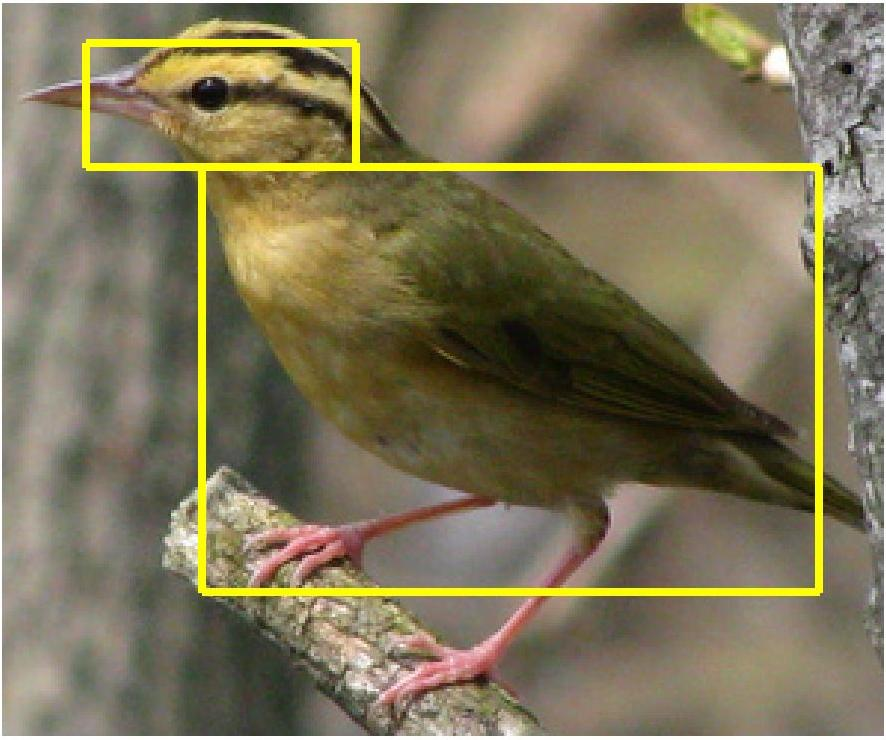
\includegraphics[width=0.15\linewidth, height = 0.1\linewidth]{8_5.jpg} 
\end{center}
\caption{{Illustration of geometric constant $\delta^{NP}$. In each row, the first column is the test image with an R-CNN bounding box detection, and the rest are the top-five nearest neighbors in the training set, indexed using \texttt{pool5} features and cosine distance metric.}}
\label{fig:np}
\end{figure*}


%
%\begin{figure*}[t]
%\begin{center}
%\includegraphics[height=0.30\linewidth]{bird_img_head_keypoints.pdf}
%\includegraphics[height=0.30\linewidth]{bird_img_body_keypoints.pdf}
%\end{center}
%\caption{{Definition of head and body bird parts.  Left image shows keypoints which comprise the head part. Right image shows the keypoints which comprise the body part.}}
%\label{fig:ningfig}
%\end{figure*}

\subsection{Fine-grained categorization}
We extract semantic features from localized parts as well as the whole object. The final feature representation is $[\phi(x_0) \ldots \phi(x_n)]$ where $x_0$ and $x_{1 \ldots n}$ are whole-object and part location predictions inferred using one of the models from the previous section and $\phi(x_i)$ is the feature representation of part $x_i$.

In one set of experiments, we extract deep convolutional features $\phi(x_i)$ from an ImageNet pre-trained CNN, similar to DeCAF~\cite{decaf}.
In order to make the deep CNN-derived features more discriminative for the target task of fine-grained bird classification, we also fine-tune the ImageNet pre-trained CNN for the 200-way bird classification task from ground truth bounding box crops of the original CUB images.
In particular, we replace the original 1000-way \texttt{fc8} classification layer with a new 200-way \texttt{fc8} layer with randomly initialized weights drawn from a Gaussian with $\mu = 0$ and $\sigma = 0.01$.
We set fine-tuning learning rates as proposed by R-CNN~\cite{rcnn}, initializing the global rate to a tenth of the initial ImageNet learning rate and dropping it by a factor of 10 throughout training, but with a learning rate in the new \texttt{fc8} layer of 10 times the global learning rate.
For the whole object bounding box and each of the part bounding boxes, we independently finetune the ImageNet pre-trained CNN for classification on ground truth crops of each region warped to the $227 \times 227$ network input size, always with 16 pixels on each edge of the input serving as context as in R-CNN~\cite{rcnn}.
At test time, we extract features for the predicted whole object or part region using the network fine-tuned for that particular whole object or part.

%We use the same deep convolutional features for classification as used for object detection and part localization. 
For training the classifier, we employ a one-versus-all linear SVM using the final feature representation. For a new test image, we apply the whole and part detectors with the geometric scoring function to get detected part locations and use the features for prediction.
If a particular part $i$ was not detected anywhere in the test image (due to all proposals falling below the part detector's threshold, set to achieve high recall), we set its features $\phi(x_i) = \mathbf{0}$ (zero vector).
